


% =====================================================================
%  Phase 3 / Phase 4 -- ztachip on Zynq-7000 ZC702
%  Expanded version with diagrams (TikZ/pgfplots) and tables.
%
%  REQUIRED PACKAGES (add to your main preamble if not already present):
%     \usepackage{booktabs}      % \toprule \midrule \bottomrule
%     \usepackage{array}         % m{} column type
%     \usepackage{graphicx}      % \resizebox
%     \usepackage{float}         % [H] float placement
%     \usepackage{siunitx}       % aligned numbers (optional but used below)
%     \usepackage{tikz}
%     \usetikzlibrary{positioning,arrows.meta,shapes.geometric,calc,fit,backgrounds}
%     \usepackage{pgfplots}
%     \pgfplotsset{compat=1.18}
%
%  If your "prism" template already loads these, delete the duplicates.
% =====================================================================


\section{Phase 3: Successful Deployment---ARM as Clock and DDR Source Only}

\subsection{Architectural Pivot and Design Philosophy}

The successful deployment returned to the original ztachip philosophy: the soft-core
\texttt{VexRiscv} RISC-V processor is the \emph{sole active processor} during inference. The hard
ARM Processing System (PS) is configured but runs no user application; its only roles are
\emph{passive}: it supplies the fabric clocks (FCLK) and grants the Programmable Logic (PL) access
to DDR memory through the 64-bit High-Performance AXI slave port (\texttt{S\_AXI\_HP0}). During
bring-up, the host PC uses JTAG to (i) run the Xilinx-provided \texttt{ps7\_init} sequence,
(ii) load firmware and model data into DDR, (iii) initialise the console mailbox, and (iv) release
VexRiscv from reset. From that point VexRiscv runs independently with no ARM involvement.

This architecture removed four sources of fragility that defeated earlier attempts: the custom ARM
loader, the \texttt{SYSCTRL} reset dependency, the SD-card / FatFs dependency, and the active
ARM$\leftrightarrow$VexRiscv software hand-shaking. The only ARM-side code that executes is the
board-specific \texttt{ps7\_init} routine generated from the Vivado PS configuration.

Figure~\ref{fig:p3-arch} shows the resulting partitioning. Table~\ref{tab:p3-mapping} summarises
how each Arty~A7 facility was re-mapped onto the ZC702.

% ---------------------------------------------------------------------
% Figure: system architecture / partitioning
% ---------------------------------------------------------------------
\begin{figure}[H]
\centering
\begin{tikzpicture}[font=\small,>=Latex,
  ps/.style   ={draw,rounded corners,fill=orange!10,align=center,minimum height=9mm,minimum width=27mm},
  pl/.style   ={draw,rounded corners,fill=blue!8,align=center,minimum height=9mm,minimum width=31mm},
  host/.style ={draw,rounded corners,fill=gray!12,align=center,minimum height=9mm,minimum width=24mm},
  ddr/.style  ={draw,rounded corners,fill=green!10,align=center,minimum height=9mm,minimum width=27mm},
  lbl/.style  ={font=\scriptsize\itshape}]

% --- Host
\node[host] (host) at (0,-0.1) {Host PC\\\scriptsize \texttt{xsdb} over USB-JTAG};

% --- PS column (x=5.5)
\node[ps]  (ps7)  at (5.5,1.5)  {\texttt{ps7\_init}\\\scriptsize clocks, DDR, MIO};
\node[ps]  (fclk) at (5.5,0.0)  {FCLK 93.75\,MHz};
\node[ddr] (ddr)  at (5.5,-1.7) {DDR Controller\\\scriptsize 1\,GB, 64-bit};

% --- PL column (x=11.5)
\node[pl] (mmcm) at (11.5,1.5)  {MMCM\\\scriptsize 93.75 \& 187.5\,MHz};
\node[pl] (vex)  at (11.5,0.0)  {VexRiscv\\\scriptsize rv32im control CPU};
\node[pl] (zta)  at (11.5,-1.7) {ztachip tensor engine\\\scriptsize Pcores + FPU + dataplane};

% --- enclosing boxes
\begin{scope}[on background layer]
  \node[draw,dashed,rounded corners,fill=orange!4,inner sep=5mm,fit=(ps7)(fclk)(ddr),
        label={[lbl]above:Processing System (PS) --- passive}] (psbox) {};
  \node[draw,dashed,rounded corners,fill=blue!3,inner sep=5mm,fit=(mmcm)(vex)(zta),
        label={[lbl]above:Programmable Logic (PL) --- active}] (plbox) {};
\end{scope}

% --- arrows (labels kept in empty space; clock & control run vertically inside PL)
\draw[->]  (host.east) -- (psbox.west) node[midway,above,lbl]{JTAG};
\draw[->]  (fclk.east) -- (mmcm.west) node[pos=0.5,sloped,above=1pt,lbl]{1 clock root};                                                                                            \draw[<->] (ddr.east)  -- (zta.west)  node[midway,below=1pt,lbl]{S\_AXI\_HP0 (64-bit)};
\draw[->]  (mmcm) -- (vex) node[midway,right=1pt,lbl]{clk};
\draw[->]  (vex)  -- (zta) node[midway,right=1pt,lbl]{control};
\end{tikzpicture}
\caption{Phase~3 partitioning. The PS provides only clocks and DDR; all computation runs in the PL
on VexRiscv and the ztachip tensor engine. The host participates only at bring-up over JTAG.}
\label{fig:p3-arch}
\end{figure}

\begin{table}[H]
\centering
\caption{Platform re-mapping from the Arty~A7 reference to the ZC702 (Phase~3).}
\label{tab:p3-mapping}
\renewcommand{\arraystretch}{1.2}
\begin{tabular}{@{}lll@{}}
\toprule
\textbf{Facility} & \textbf{Arty A7 (reference)} & \textbf{ZC702 (this work)} \\
\midrule
FPGA device        & XC7A100T (Artix-7)        & XC7Z020 (Zynq-7000) \\
Memory controller  & Soft MIG (external DDR3)   & Hard PS DDR controller via \texttt{S\_AXI\_HP0} \\
Memory data width  & 128-bit                    & 64-bit (\texttt{exmem\_data\_width\_c}=64) \\
Clock source       & Oscillator + Clk.\ Wizard  & One PS FCLK $\rightarrow$ MMCM (2:1) \\
Model transport    & Ethernet (TFTP)            & JTAG pre-load into DDR \\
Console I/O        & UART                       & DDR mailbox ring buffer over JTAG \\
Active processor   & VexRiscv                   & VexRiscv (ARM passive) \\
\bottomrule
\end{tabular}
\end{table}


\subsection{Clock Architecture Correction: MMCM for Exact 2:1 Ratio}
\label{subsec:p3-clock}

ztachip requires the dataplane double-rate clock \texttt{clk\_x2} to be \emph{exactly} twice the
main clock frequency, because parts of the dataplane emit two words per main-clock cycle. The Zynq
PS derives its FCLK outputs by integer division of an internal 1500\,MHz PLL, so an exact 2:1 pair
is available only where both divisors are integral. The pair
$93.75\,\text{MHz} = 1500/16$ and $187.5\,\text{MHz} = 1500/8$ satisfies this and sits just below
100\,MHz, leaving timing margin (Table~\ref{tab:p3-clocks}).

\begin{table}[H]
\centering
\caption{Clock selection. Both frequencies are exact integer divisions of the 1500\,MHz PS PLL,
guaranteeing a precise 2:1 ratio.}
\label{tab:p3-clocks}
\renewcommand{\arraystretch}{1.2}
\begin{tabular}{@{}lccc@{}}
\toprule
\textbf{Clock} & \textbf{Role} & \textbf{Divisor of 1500\,MHz} & \textbf{Frequency} \\
\midrule
\texttt{clk\_main} & Main fabric / control & $\div 16$ & 93.75\,MHz \\
\texttt{clk\_x2}   & Dataplane double-rate & $\div 8$  & 187.5\,MHz \\
\bottomrule
\end{tabular}
\end{table}

The earlier design drove the two clocks from \emph{two independent} FCLK outputs, which Vivado
treated as unrelated clock roots. This produced \emph{hold} violations that --- as explained in
Section~\ref{subsec:p3-crpr} --- could not be removed by changing the clock frequency. The final
design (Figure~\ref{fig:p3-clock}) instead routes a \emph{single} 93.75\,MHz FCLK into the PL and
feeds it to a Mixed-Mode Clock Manager (MMCM) generated by the Clocking Wizard. The MMCM synthesises
\emph{both} 93.75\,MHz and 187.5\,MHz from one common node, giving the two clocks the shared root the
analyser needs to relax the hold checks.

\begin{figure}[H]
\centering
\begin{tikzpicture}[font=\small,>=Latex,
  blk/.style={draw,rounded corners,minimum height=8mm,minimum width=15mm,align=center},
  captionnote/.style={font=\scriptsize\itshape}]

% ---- LEFT: failing two-root scheme (centred on y=0) ----
\node[blk,fill=red!6]  (f1) at (0,0.75)  {FCLK0\\\scriptsize 93.75\,MHz};
\node[blk,fill=red!6]  (f2) at (0,-0.75) {FCLK1\\\scriptsize 187.5\,MHz};
\node[blk,fill=red!10] (l1) at (3,0)     {ztachip\\\scriptsize logic};
\draw[->] (f1.east) -- (l1.west |- f1);
\draw[->] (f2.east) -- (l1.west |- f2);
\node[captionnote,align=center] at (1.5,1.8) {Two independent roots\\(failed)};
\node[captionnote,red!60!black,align=center] at (1.5,-1.9)
  {Independent roots $\Rightarrow$ no CRPR\\$\Rightarrow$ hold violations};

% ---- divider ----
\draw[dashed,gray] (5.4,-2.3) -- (5.4,2.2);

% ---- RIGHT: single-root MMCM scheme (centred on y=0) ----
\node[blk,fill=green!8]  (fc)   at (7,0)      {FCLK\\\scriptsize 93.75\,MHz};
\node[blk,fill=green!12] (mmcm) at (9.3,0)    {MMCM};
\node[blk,fill=green!8]  (o1)   at (11.4,0.8) {\scriptsize 93.75\,MHz};
\node[blk,fill=green!8]  (o2)   at (11.4,-0.8){\scriptsize 187.5\,MHz};
\node[blk,fill=green!10] (l2)   at (13.7,0)   {ztachip\\\scriptsize logic};
\draw[->] (fc)   -- (mmcm);
\draw[->] (mmcm) -- (o1);
\draw[->] (mmcm) -- (o2);
\draw[->] (o1.east) -- (l2.west |- o1);
\draw[->] (o2.east) -- (l2.west |- o2);
\node[captionnote,align=center] at (10.3,1.8) {Single MMCM root\\(adopted)};
\node[captionnote,green!45!black,align=center] at (10.3,-1.9)
  {Common root $\Rightarrow$ CRPR applies\\$\Rightarrow$ timing closes};
\end{tikzpicture}
\caption{Left: the failing two-root scheme. Right: the adopted single-root MMCM scheme that
generates both clocks from a common node and closes timing.}
\label{fig:p3-clock}
\end{figure}

\subsection{Why the Hold Violation Arose: Clock-Reconvergence Pessimism}
\label{subsec:p3-crpr}

The clock change of the previous section was driven by a specific static-timing-analysis (STA)
failure that is worth explaining in its own right, because it is a common and counter-intuitive
trap. STA verifies two kinds of constraint at every flip-flop pair. A \emph{setup} check requires
that data launched by one clock edge arrive at the capturing flip-flop \emph{before} the next active
edge; it is relaxed by slowing the clock. A \emph{hold} check requires that data launched by an edge
\emph{not} arrive so soon that it races through and corrupts the capturing flip-flop on the
\emph{same} edge; because launch and capture happen on the same edge, a hold check is independent of
clock period and \textbf{cannot be fixed by lowering the frequency}. The violations encountered here
were hold violations, which is why a structural clocking change --- not a slower clock --- was
required.

To be safe, STA adds a guard band of \emph{clock uncertainty} (jitter plus skew) to every check. For
a hold check it charges this uncertainty pessimistically, as though the launch and capture clocks
could drift apart by the full amount. In reality, the launch and capture clocks usually travel
together through a shared early portion of the clock tree --- the same source buffers and routing ---
before diverging to their respective flip-flops (Figure~\ref{fig:p3-crpr}). Uncertainty on that
\emph{common} segment affects both flip-flops identically and therefore cannot cause them to drift
relative to one another. \emph{Clock-Reconvergence Pessimism Removal} (CRPR) is the STA step that
credits this shared portion back, removing the double-counted pessimism and relaxing the hold
requirement to a realistic value.

\begin{figure}[H]
\centering
\begin{tikzpicture}[font=\scriptsize,>=Latex,
  ff/.style={draw,fill=blue!6,minimum width=9mm,minimum height=12mm,align=center},
  buf/.style={draw,fill=gray!12,regular polygon,regular polygon sides=3,rotate=-90,minimum size=6mm,inner sep=0pt},
  cl/.style={draw,fill=green!10,ellipse,minimum width=15mm,minimum height=9mm}]

% --- clock trunk (bottom): CLK -> b1 -> b2; branch is b2's output tip ---
\node (clk) at (0,-1) {CLK};
\node[buf] (b1) at (1.1,-1) {};
\node[buf] (b2) at (2.4,-1) {};
\coordinate (P) at (b2.east);   % branch point = the buffer's output tip
\draw[->] (clk) -- (b1);
\draw[->] (b1) -- (b2);
\fill (P) circle (1.4pt);

% --- flip-flops/logic: Launch FF placed DIRECTLY above the branch point ---
\node[ff] (L)     at ([yshift=25mm]P) {Launch\\FF};
\node[cl] (cloud) at ([xshift=22mm]L) {logic};
\node[ff] (C)     at ([xshift=22mm]cloud) {Capture\\FF};
\draw[->] (L.east) -- (cloud.west);
\draw[->] (cloud.east) -- (C.west);
\node[font=\scriptsize\itshape] at ([yshift=9mm]cloud.north) {data path};

% --- clock branches, both originating at the buffer tip P ---
\draw[->] (P) -- (L.south);                % straight up to launch FF (vertical)
\node[buf] (b3) at ([xshift=24mm]P) {};    % capture-path buffer on the clock line
\draw[->] (P) -- (b3);                     % right into b3's input (base)
\draw[->] (b3.east) -| (C.south);          % b3 output tip up to capture FF

% label pointing at the actual branch-point dot
\node[font=\scriptsize\itshape] (bplbl) at (1.55,-0.3) {branch point};
\draw[gray,-{Latex[length=4pt]}] (bplbl.east) -- (P);

% --- bracket marking the common clock path ---
\draw[green!45!black,thick] ([yshift=-5mm]clk.south) -- ([yshift=-5mm]P);
\draw[green!45!black,thick] ([yshift=-3.5mm]clk.south) -- ([yshift=-6.5mm]clk.south);
\draw[green!45!black,thick] ([yshift=-3.5mm]P) -- ([yshift=-6.5mm]P);
\node[green!45!black,align=center,below=1mm] at ($([yshift=-5mm]clk.south)!0.5!([yshift=-5mm]P)$)
  {common clock path --- CRPR credits this segment back};
\end{tikzpicture}
\caption{Clock-reconvergence pessimism. The launch and capture clocks share a common early path
(\texttt{CLK} through the source buffers to the branch point); only beyond it do they diverge.
Uncertainty on the shared segment moves both flip-flops together and must not be charged against the
hold check --- CRPR removes it.}
\label{fig:p3-crpr}
\end{figure}

With two independent \texttt{FCLK} outputs the launch and capture clock trees had \emph{no} common
node: each clock originated at a separate PS output. STA could therefore apply no CRPR credit and
charged the full uncertainty against every hold path, producing the three hold violations. Routing a
single \texttt{FCLK} into one MMCM (Section~\ref{subsec:p3-clock}) gives both derived clocks a shared
root, so the common-path credit is restored; with the input-jitter constraint refined, all hold
checks then passed, and the design closed with worst negative slack $0.000$\,ns and worst hold slack
$+0.009$\,ns.





\subsection{Firmware Architecture: Split Binary and OCM Boot Stub}

The VexRiscv reset vector is hardwired to \texttt{0x00004000}. When the Zynq On-Chip Memory (OCM) is
mapped to low addresses, that address falls inside OCM. A small vector stub
(code+data on the order of a few hundred bytes; the emitted binary is $\approx 0.5$\,KB) is loaded at
\texttt{0x00004000}; it initialises the global and stack pointers and jumps to the main firmware in
DDR at \texttt{0x00100000}. The main firmware binary is $\approx 8.4$\,MiB ($\approx 8.8$\,MB) and
contains the C runtime, the ztachip application framework, and the LLM inference code.

The split layout (Figure~\ref{fig:p3-mem}) serves two purposes. First, it straddles the Zynq
low-memory reserved gap \texttt{0x00040000}--\texttt{0x000FFFFF}, which is not writable through the
debug interface on this device. Second, it lets the boot target change \emph{without} rebuilding
VexRiscv: only the tiny startup stub lives in OCM, while the full firmware lives in DDR. The linker
script defines separate OCM and DDR regions accordingly.

% ---------------------------------------------------------------------
% Figure: memory map (vertical address space)
% ---------------------------------------------------------------------
\begin{figure}[H]
\centering
\begin{tikzpicture}[font=\scriptsize,
  seg/.style={draw,text width=60mm,align=center,minimum height=9mm,outer sep=0pt},
  addr/.style={font=\scriptsize\ttfamily,anchor=east}]
% --- stack from low (bottom) to high (top) address; 0pt gaps so edges meet ---
\node[seg,fill=gray!12]  (tcm)  at (0,0) {PL BRAM / TCM --- stack, scratch};
\node[seg,fill=blue!10,  above=0pt of tcm]  (ocm) {PS OCM (mapped low) --- vector stub @ \texttt{0x00004000}};
\node[seg,fill=red!12,   above=0pt of ocm]  (gap) {Reserved gap (not debug-writable)};
\node[seg,fill=green!12, above=0pt of gap,minimum height=11mm] (fw) {Firmware main image @ \texttt{0x00100000} ($\approx$8.4\,MiB)};
\node[seg,fill=green!6,  above=0pt of fw,minimum height=11mm]  (heap) {Firmware heap / KV-cache / activations / logits};
\node[seg,fill=yellow!20,above=0pt of heap] (model) {Model ZUF @ \texttt{0x10000000} --- marker ``ZTAC''};
\node[seg,fill=orange!18,above=0pt of model] (mbx) {Mailbox console @ \texttt{0x30000000} --- marker ``ZTCH''};
% --- address labels anchored to each box's bottom boundary (cannot drift) ---
\node[addr] at ([xshift=-2mm]tcm.south west)   {0x00000000};
\node[addr] at ([xshift=-2mm]ocm.south west)   {0x00004000};
\node[addr] at ([xshift=-2mm]gap.south west)   {0x00040000};
\node[addr] at ([xshift=-2mm]fw.south west)    {0x00100000};
\node[addr] at ([xshift=-2mm]model.south west) {0x10000000};
\node[addr] at ([xshift=-2mm]mbx.south west)   {0x30000000};
% --- "higher addresses" arrow on the RIGHT, clear of the labels and boxes ---
\draw[->] ([xshift=4mm]tcm.south east) -- ([xshift=4mm]mbx.north east)
  node[midway,rotate=-90,anchor=south,font=\scriptsize]{higher addresses};
\end{tikzpicture}
\caption{Phase~3 DDR/OCM memory map. The firmware is split across the reserved low-memory gap; the
model and mailbox occupy distinct high-address regions. (The mailbox was relocated from
\texttt{0x20000000} to \texttt{0x30000000} so the 308\,MB SmolLM2-360M model would fit below it.)}
\label{fig:p3-mem}
\end{figure}

\begin{table}[H]
\centering
\caption{Consolidated address map (current board scripts).}
\label{tab:p3-memmap}
\renewcommand{\arraystretch}{1.2}
\begin{tabular}{@{}lll@{}}
\toprule
\textbf{Address} & \textbf{Contents} & \textbf{Notes} \\
\midrule
\texttt{0x00000000}--\texttt{0x00003FFF} & PL BRAM / TCM   & stack \& scratch \\
\texttt{0x00004000}                      & Vector stub (OCM) & reset vector; $\approx 0.5$\,KB \\
\texttt{0x00040000}--\texttt{0x000FFFFF} & Reserved gap    & not writable via debug \\
\texttt{0x00100000}                      & Firmware main image & $\approx 8.4$\,MiB \\
\texttt{0x10000000}                      & Model ZUF       & marker ``ZTAC'' (\texttt{0x4341545A}) \\
\texttt{0x30000000}                      & Mailbox console & marker ``ZTCH'' (\texttt{0x5A544348}) \\
\bottomrule
\end{tabular}
\end{table}

\subsection{Model Delivery via JTAG Pre-Loading}

Ethernet delivery was replaced by JTAG pre-loading. The SmolLM2-135M ZUF file
($\approx 141$--$147$\,MB depending on regeneration) is written into DDR at \texttt{0x10000000}
through the Xilinx \texttt{xsdb} memory-write interface. A magic word at the file start---the ASCII
string ``ZTAC'' stored little-endian (\texttt{0x4341545A})---lets the boot script \emph{skip} the
transfer when the model is already resident, cutting subsequent boot time from $\approx 40$ minutes
to under one minute (Table~\ref{tab:p3-load}). The model is placed at the 256\,MB offset
(\texttt{0x10000000}) to avoid collision with the firmware heap, the key/value cache, the activation
tensors, and the output-logit buffers. Because the JTAG link is per-transaction-latency bound
($\approx 65$\,KB/s), a single large write was found to silently under-transfer; a \emph{chunked}
write with read-back verification is used instead.

\begin{table}[H]
\centering
\caption{JTAG model-load time by configuration (cold load; warm boot skips via the ``ZTAC'' magic).}
\label{tab:p3-load}
\renewcommand{\arraystretch}{1.2}
\begin{tabular}{@{}lcc@{}}
\toprule
\textbf{Model} & \textbf{File size} & \textbf{Approx.\ cold-load time} \\
\midrule
SmolLM2-135M Q4 & 147\,MB & $\sim$38--40\,min \\
SmolLM2-135M Q8 & 200\,MB & $\sim$52\,min \\
SmolLM2-360M Q4 & 308\,MB & $\sim$88\,min \\
\bottomrule
\end{tabular}
\end{table}

\subsection{DDR Mailbox Console: Substituting for the Unavailable UART}

On the ZC702 the USB-to-serial bridge connects to the \emph{PS} UART, not to PL pins, so VexRiscv
cannot reach it in the Phase~3 partitioning. A DDR mailbox ring buffer was implemented instead, at
\texttt{0x30000000}.\footnote{The mailbox originally resided at \texttt{0x20000000}; it was moved to
\texttt{0x30000000} so the 308\,MB SmolLM2-360M model could occupy the 512\,MB region below it. All
current board scripts use \texttt{0x30000000}.} It contains a magic word, head/tail pointers, and two
4\,KB ring buffers---one chip$\rightarrow$PC and one PC$\rightarrow$chip (Figure~\ref{fig:p3-mbx}).

VexRiscv firmware routes \texttt{printf} into the chip$\rightarrow$PC ring and reads keystrokes from
the PC$\rightarrow$chip ring. A host-side TCL script under \texttt{xsdb} polls the output ring and
prints characters to the terminal, while typed input is pushed into the input ring. Two reliability
fixes were required: (i) the host boot script clears stale pointer values from previous sessions
before releasing VexRiscv; and (ii) \texttt{xsdb} context invalidation during long polling is handled
by wrapping each memory access in a TCL exception handler that re-selects and halts the ARM core
before retrying.

\begin{figure}[H]
\centering
\begin{tikzpicture}[font=\scriptsize,>=Latex,
  cell/.style={draw,minimum width=10mm,minimum height=7mm},
  ringo/.style={draw,fill=blue!8,minimum width=46mm,minimum height=8mm,align=center},
  ringi/.style={draw,fill=orange!12,minimum width=46mm,minimum height=8mm,align=center},
  hdr/.style={draw,fill=gray!12,minimum width=46mm,minimum height=7mm,align=center}]
\node[hdr]  (magic) at (0,2.4) {magic ``ZTCH'' \;|\; out.head \; out.tail \;|\; in.head \; in.tail};
\node[ringo] (o) at (0,1.2) {chip $\rightarrow$ PC ring (4\,KB)};
\node[ringi] (i) at (0,0.0) {PC $\rightarrow$ chip ring (4\,KB)};
\node[draw,fill=blue!4,left=10mm of o,align=center,minimum height=8mm] (vex) {VexRiscv\\\texttt{printf}};
\node[draw,fill=orange!6,right=10mm of i,align=center,minimum height=8mm] (host){Host\\\texttt{xsdb} poll};
\draw[->] (vex.east) -- (o.west) node[midway,above]{write};
\draw[->] (o.east) -| ([xshift=6mm]o.east) |- (host.north west) node[pos=0.25,right]{read};
\draw[->] (host.south west) |- (i.east) node[pos=0.75,below]{write};
\draw[->] (i.west) -| ([xshift=-6mm]i.west) |- (vex.south east) node[pos=0.25,left]{read};
\end{tikzpicture}
\caption{DDR mailbox: a header (magic + head/tail indices) plus two 4\,KB ring buffers carrying
console output and input between VexRiscv and the host over JTAG.}
\label{fig:p3-mbx}
\end{figure}

\subsection{The Critical Bug: VexRiscv Misaligned Memory-Access Trap}

After booting and reading the model header, the system initially froze while parsing model
configuration keys. Checkpoint prints localised the freeze to the ZUF parser's key-lookup function.
The root cause was a \emph{misaligned memory-access trap} triggered by optimised standard-C string
routines operating on raw model-file strings.

VexRiscv implements \texttt{rv32im} and provides \emph{no} hardware support for misaligned word
loads. A compiler-optimised \texttt{strcmp} reads four bytes at a time, but ZUF key strings are not
guaranteed to be four-byte aligned. A word load from an address such as \texttt{0x10000031}
(Figure~\ref{fig:p3-trap}) raises a misaligned-access exception; with no handler installed, the core
vectored to address~0 and effectively halted---silently, with no diagnostic.

The fix replaced library string comparison on raw model bytes with custom \emph{byte-by-byte}
comparisons (inherently aligned), applied at the ZUF parser and tokeniser comparison sites. After
the fix, model loading completed through all configuration keys and the 49{,}152 vocabulary entries,
and the LLM inference loop initialised correctly. The resulting design rule---\emph{never apply
word-optimised string routines to unaligned DDR model bytes}---is recorded for future work.

\begin{figure}[H]
\centering
\begin{tikzpicture}[font=\scriptsize,>=Latex,
  byte/.style={draw,minimum width=9mm,minimum height=7mm,align=center,font=\scriptsize\ttfamily},
  tag/.style={align=left,font=\scriptsize}]

% header note
\node[font=\scriptsize\itshape] at (3.0,2.35)
  {32-bit word loads on \texttt{rv32im} must start on a 4-byte boundary (offset 0, 4, 8, \dots).};

% --- aligned row (top): word covers bytes ..30--..33 ---
\foreach \x/\lab/\f in {0/30/green!22,1/31/green!22,2/32/green!22,3/33/green!22,4/34/white,5/35/white,6/36/white,7/37/white}
  \node[byte,fill=\f] (t\x) at (\x*0.95,1.25) {..\lab};
\node[tag,green!45!black,left=4mm of t0]  {aligned\\start \texttt{..30}};
\node[tag,green!45!black,right=4mm of t7] {$\Rightarrow$ one word, \textbf{OK}};

% --- misaligned row (bottom): word covers bytes ..31--..34 ---
\foreach \x/\lab/\f in {0/30/white,1/31/red!20,2/32/red!20,3/33/red!20,4/34/red!20,5/35/white,6/36/white,7/37/white}
  \node[byte,fill=\f] (m\x) at (\x*0.95,0) {..\lab};
\node[tag,red!60!black,left=4mm of m0]  {misaligned\\start \texttt{..31}};
\node[tag,red!60!black,right=4mm of m7] {$\Rightarrow$ \textbf{TRAP}};
\end{tikzpicture}
\caption{Word loads must be four-byte aligned on \texttt{rv32im}. A \texttt{strcmp} that reads a word
starting at an odd offset (e.g.\ \texttt{0x10000031}) traps; byte-wise comparison avoids it.}
\label{fig:p3-trap}
\end{figure}

\subsection{Complete System Bring-up Sequence}

The validated bring-up sequence is summarised in Figure~\ref{fig:p3-boot}. The host connects over
USB-JTAG, launches \texttt{xsdb}, and selects the ARM target; \texttt{ps7\_init} and
\texttt{ps7\_post\_config} then configure DDR, clocks, and MIO. VexRiscv is held in reset through the
PS-controlled \texttt{FPGA\_RST\_CTRL} \emph{before} the PL is brought up, and all OCM blocks are
mapped low so that \texttt{0x00000000}--\texttt{0x0003FFFF} form one contiguous region. Only then is
the PL bitstream programmed. The boot script next checks the model magic word and loads the model
only if absent, writes the vector stub to \texttt{0x00004000} and the main firmware to
\texttt{0x00100000}, zeros the mailbox region, and finally releases VexRiscv from reset, after which
the host polls the mailbox console. The ARM core itself takes no part---it remains halted under the
debugger throughout. VexRiscv boots from the OCM stub, jumps to \texttt{crtInit} in DDR, performs
C-runtime initialisation, calls \texttt{main}, opens the model, builds the tokeniser, and prints the
startup banner and prompt into the mailbox.

\noindent\textbf{Operational constraint.} The system boots reliably only on the \emph{first}
bring-up after a power cycle; re-initialising an already-running PS can leave it inconsistent (silent
no-boot, or an ``AHB AP transaction error / blocked address \texttt{0x4000}'' on the OCM write).
A power cycle therefore precedes every fresh run.

\begin{figure}[H]
\centering
\begin{tikzpicture}[font=\scriptsize,>=Latex,node distance=4mm and 8mm,
  bootstep/.style={draw,rounded corners,fill=blue!6,align=center,text width=46mm,inner sep=3pt,minimum height=7mm},
  vex/.style ={draw,rounded corners,fill=green!8,align=center,text width=40mm,inner sep=3pt,minimum height=7mm}]
\node[bootstep] (s1) {1. Connect JTAG, launch \texttt{xsdb}; select ARM};
\node[bootstep,below=of s1] (s2) {2. \texttt{ps7\_init} / \texttt{ps7\_post\_config}\\\scriptsize DDR, clocks, MIO};
\node[bootstep,below=of s2] (s3) {3. Hold VexRiscv in reset\\\scriptsize \texttt{FPGA\_RST\_CTRL}=1};
\node[bootstep,below=of s3] (s4) {4. Map all OCM blocks low\\\scriptsize contiguous \texttt{0x0}--\texttt{0x3FFFF}};
\node[bootstep,below=of s4] (s5) {5. Program PL bitstream};
\node[bootstep,below=of s5] (s6) {6. Check ``ZTAC''; load model if absent;\\ write stub @ \texttt{0x4000}, firmware @ \texttt{0x100000}};
\node[bootstep,below=of s6] (s7) {7. Zero mailbox; release VexRiscv\\\scriptsize \texttt{FPGA\_RST\_CTRL}=0};
\node[vex,right=26mm of s4] (v1) {VexRiscv: OCM stub $\rightarrow$ \texttt{crtInit}};
\node[vex,below=of v1] (v2) {C-runtime init $\rightarrow$ \texttt{main}};
\node[vex,below=of v2] (v3) {Open model, build tokeniser};
\node[vex,below=of v3] (v4) {Print banner \& prompt to mailbox};
\foreach \a/\b in {s1/s2,s2/s3,s3/s4,s4/s5,s5/s6,s6/s7} \draw[->] (\a)--(\b);
\foreach \a/\b in {v1/v2,v2/v3,v3/v4} \draw[->] (\a)--(\b);
\draw[->,dashed] (s7.east) -- ++(6mm,0) |- (v1.west) node[pos=0.25,right,font=\scriptsize\itshape]{release};
\end{tikzpicture}
\caption{Bring-up flow. Left column: host actions over JTAG. Right column: autonomous VexRiscv boot
after release. ARM takes no part once VexRiscv is running.}
\label{fig:p3-boot}
\end{figure}

\subsection{On-Silicon Functional Verification of the Compute Kernels}

Before entrusting the accelerator with a full model, every ztachip LLM compute kernel was verified on
the board against a bit-exact reference C implementation (\texttt{llm\_ref.c}) using a dedicated lean
firmware build. Each kernel ran on self-generated operands and its output was compared element by
element; correctness required \emph{zero} mismatches. This verification is performed on silicon
rather than in RTL simulation because the heavy INT4/INT8 matrix-multiply kernels need on the order of
$10^{9}$ cycles and are intractable to simulate (hours each), yet complete in seconds on the device.
All eleven kernels matched the reference exactly (Table~\ref{tab:p3-kernels}).

\begin{table}[H]
\centering
\caption{On-silicon kernel self-test (XC7Z020 @ 93.75\,MHz). Every kernel matched the bit-exact
reference with zero mismatches.}
\label{tab:p3-kernels}
\renewcommand{\arraystretch}{1.15}
\begin{tabular}{@{}rlrr@{}}
\toprule
\textbf{\#} & \textbf{Kernel} & \textbf{Elements compared} & \textbf{Mismatches} \\
\midrule
1 & residual          & 1{,}152  & 0 \\
2 & SwiGLU            & 1{,}536  & 0 \\
3 & rms               & 1{,}152  & 0 \\
4 & rope              & 384      & 0 \\
5 & softmax           & 512      & 0 \\
6 & k\_max            & 1        & 0 \\
7 & cosine            & 14{,}400 & 0 \\
8 & sine              & 14{,}400 & 0 \\
9 & quantize          & 2{,}048  & 0 \\
10 & \textbf{matmul\_q4} & 1{,}536 & 0 \\
11 & \textbf{matmul\_q8} & 1{,}536 & 0 \\
\midrule
\multicolumn{2}{l}{\textbf{Total}} & \textbf{38{,}657} & \textbf{0} \\
\bottomrule
\end{tabular}
\end{table}

\subsection{FPGA Resource Utilisation}

Table~\ref{tab:p3-util} reports the post-implementation utilisation. The high LUT and BRAM occupancy
($\approx 86\%$ and $\approx 94\%$) confirms that the integrated design substantially fills this
small device, which motivated the compact ztachip configuration and the choice of a small model.
Two further figures are worth noting: occupied slices reach approximately 99\%, indicating the fabric
is almost fully populated; and exactly one of the four MMCMs is instantiated --- the single common
clock root introduced in the clock-architecture correction (Section~\ref{subsec:p3-clock}).

\begin{table}[H]
\centering
\caption{Post-implementation resource utilisation on the XC7Z020 (Vivado placed-design report). The
Block RAM figure of 131.5 tiles comprises 107 RAMB36 plus 49 RAMB18 (each RAMB18 occupying half a
tile).}
\label{tab:p3-util}
\renewcommand{\arraystretch}{1.2}
\begin{tabular}{@{}lrrr@{}}
\toprule
\textbf{Resource} & \textbf{Used} & \textbf{Available} & \textbf{Utilisation} \\
\midrule
Slice LUTs (LUT)          & 45{,}869 & 53{,}200  & 86.2\,\% \\
\quad as distributed RAM (LUTRAM) & 1{,}398 & 17{,}400 & 8.0\,\% \\
Slice Registers (FF)      & 57{,}748 & 106{,}400 & 54.3\,\% \\
Block RAM tiles (BRAM)    & 131.5    & 140       & 93.9\,\% \\
DSP slices (DSP48E1)      & 82       & 220       & 37.3\,\% \\
Bonded IOB                & 2        & 200       & 1.0\,\% \\
Clock managers (MMCM)     & 1        & 4         & 25.0\,\% \\
\bottomrule
\end{tabular}
\end{table}

% ---------------------------------------------------------------------
% Figure: utilisation bar chart (matches the Vivado summary view)
% ---------------------------------------------------------------------
\begin{figure}[H]
\centering
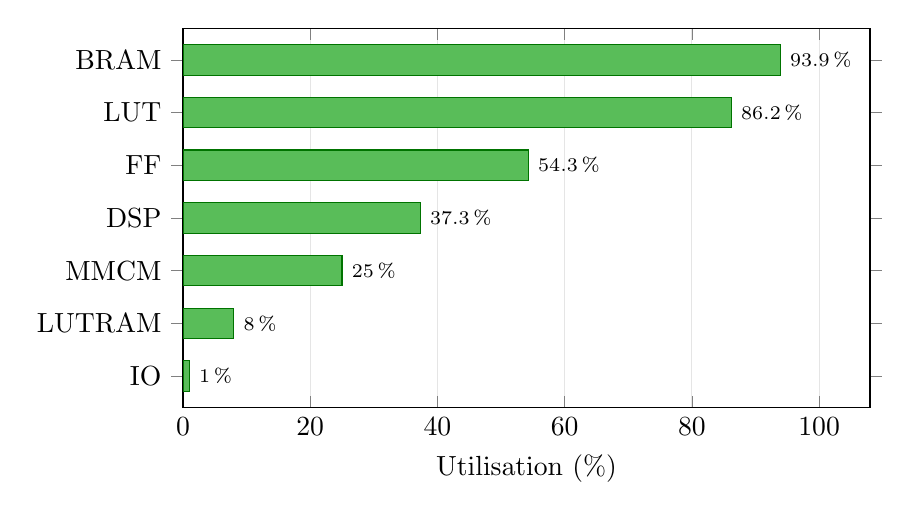
\begin{tikzpicture}
\begin{axis}[
  width=0.85\textwidth, height=6.4cm,
  xbar, bar width=11pt,
  xmin=0, xmax=108,
  xlabel={Utilisation (\%)},
  symbolic y coords={IO,LUTRAM,MMCM,DSP,FF,LUT,BRAM},
  ytick=data,
  nodes near coords={\pgfmathprintnumber[precision=1]{\pgfplotspointmeta}\,\%},
  nodes near coords style={font=\scriptsize,anchor=west},
  every axis plot/.append style={draw=green!45!black},
  enlarge y limits=0.10,
  xmajorgrids, grid style={gray!20}]
\addplot[fill=green!60!black!65] coordinates {
  (86.2,LUT) (8.0,LUTRAM) (54.3,FF) (93.9,BRAM) (37.3,DSP) (1.0,IO) (25.0,MMCM)};
\end{axis}
\end{tikzpicture}
\caption{Post-implementation resource utilisation on the XC7Z020, as a fraction of each resource's
availability. LUT ($\approx$86\,\%) and BRAM ($\approx$94\,\%) dominate, confirming that the design
nearly fills the device; the single MMCM (25\,\% of four) is the common clock root of
Section~\ref{subsec:p3-clock}.}
\label{fig:p3-util-bars}
\end{figure}

\subsection{Performance Results}

The final benchmark used 30 prompts spanning mathematics, science, geography, history, engineering,
and general knowledge. For the repository-default SmolLM2-135M~Q4 deployment, the ZC702 achieved a
mean throughput of 4.13 tokens/s and a median of 4.21 tokens/s, with a run-to-run standard deviation
of 0.29 tokens/s and an average of 213 generated tokens per run. The corresponding per-token latency
of $\approx 242$\,ms ($=1/4.13$\,s) is consistent with a memory-bandwidth-limited workload: at
93.75\,MHz over a 64-bit DDR bus with significant round-trip latency, the memory system cannot
saturate the tensor engine. The on-chip performance counters reported $\approx 103$\,MB of DDR
traffic per generated token, 431\,MB/s of DDR read bandwidth, 59\% read-engine activity, and 42.5\%
read-stall time---confirming a memory-bound rather than compute-bound deployment
(Table~\ref{tab:p3-perf}).

\paragraph{Workload design.} The 30-prompt benchmark is deliberately balanced: six topic categories
(mathematics, science, geography, history, engineering, and general knowledge) with five prompts
each. A balanced set avoids biasing the throughput figure toward any single kind of question --- for
instance, prompts that elicit very short answers would otherwise inflate the apparent token rate ---
and gives a representative spread of generation lengths. Every configuration is driven with the
\emph{identical} prompt set, so that any difference between models is attributable to the model and
its quantisation rather than to the workload.

\paragraph{Why these metrics.} The quantities in Table~\ref{tab:p3-perf} are chosen to answer a
single question: \emph{is the deployment limited by computation or by memory?} The throughput
statistics (mean, median, standard deviation) measure \emph{how fast} and \emph{how consistently}
the system generates text; the bytes-per-token, DDR-read-bandwidth, and read-active/read-stall
figures measure \emph{where the time goes}. Together they test the governing relationship of a
weight-streaming transformer,
\[
\text{throughput (tok/s)} \;=\;
\frac{\text{delivered DDR read bandwidth (MB/s)}}{\text{bytes read per token (MB)}},
\]
which holds whenever each generated token requires the model weights to be streamed once from DDR.
Were the design compute-bound, this relationship would break down --- throughput would be fixed by
the arithmetic rate and independent of the bytes moved. That it instead holds across three very
different models (the Phase~4 comparison) is the central evidence for the memory-bound conclusion.
Table~\ref{tab:p3-metrics} defines each reported quantity and the reason it is collected.

\begin{table}[H]
\centering
\caption{Definition and rationale of each performance metric reported in Table~\ref{tab:p3-perf}.}
\label{tab:p3-metrics}
\renewcommand{\arraystretch}{1.3}
\begin{tabular}{@{}>{\raggedright\arraybackslash}p{0.22\textwidth} >{\raggedright\arraybackslash}p{0.40\textwidth} >{\raggedright\arraybackslash}p{0.30\textwidth}@{}}
\toprule
\textbf{Metric} & \textbf{Meaning} & \textbf{Why it is reported} \\
\midrule
Mean throughput (tok/s) & Generated tokens divided by elapsed wall-clock time, averaged over the 30 prompts. & Primary speed measure; higher is faster. \\
Median (tok/s) & The middle throughput value across the 30 runs. & Robust to a few unusually short or long answers. \\
Std.\ deviation (tok/s) & Run-to-run dispersion of throughput. & Quantifies consistency; small values indicate near-deterministic timing. \\
Bytes per token & Weight bytes read from DDR to generate one token. & Denominator of the memory-bound model; grows with model size and precision. \\
DDR read (MB/s) & Sustained read bandwidth delivered by the memory engine. & The delivered bandwidth that bounds throughput. \\
Read-active (\%) & Fraction of cycles the read engine is actively transferring data. & Indicates how heavily the memory path is used. \\
Read-stall (\%) & Fraction of cycles a requested read is stalled, waiting on DDR. & Exposes wait time; a high value signals a memory bottleneck. \\
\bottomrule
\end{tabular}
\end{table}

\begin{table}[H]
\centering
\caption{Per-configuration throughput and memory traffic measured on the ZC702 (30-prompt workload).}
\label{tab:p3-perf}
\renewcommand{\arraystretch}{1.2}
\resizebox{\textwidth}{!}{%
\begin{tabular}{@{}lccccccc@{}}
\toprule
\textbf{Configuration} & \textbf{Mean} & \textbf{Median} & \textbf{sd} & \textbf{Bytes/} & \textbf{DDR read} & \textbf{Read} & \textbf{Read} \\
 & \textbf{(tok/s)} & \textbf{(tok/s)} & \textbf{(tok/s)} & \textbf{token} & \textbf{(MB/s)} & \textbf{active} & \textbf{stall} \\
\midrule
SmolLM2-135M Q4 & 4.13 & 4.21 & 0.29 & 103\,MB & 431 & 59\,\% & 42.5\,\% \\
SmolLM2-135M Q8 & 3.34 & 3.38 & 0.16 & 156\,MB & 526 & 71\,\% & 30\,\% \\
SmolLM2-360M Q4 & 1.90 & 1.89 & 0.04 & 248\,MB & 478 & 65\,\% & 36\,\% \\
\bottomrule
\end{tabular}}

\par\vspace{2pt}
{\footnotesize\itshape Read-active and read-stall are two independent PMU counters (the read engine's
busy fraction and its stall fraction); they are not a complementary pair and need not sum to 100\%.}
\end{table}

% =====================================================================
\section{Phase 4: Performance Comparison with NVIDIA Jetson TX1}

\subsection{Comparative Platforms}

To contextualise the ZC702 throughput, the same SmolLM2-135M family was benchmarked on an NVIDIA
Jetson TX1 (Q4\_K\_M quantisation via \texttt{llama.cpp}). The Jetson TX1 pairs a 256-core Maxwell
GPU with a quad-core ARM Cortex-A57 and 4\,GB of shared LPDDR4. Table~\ref{tab:p4-platforms} lists
the relevant platform parameters; the order-of-magnitude differences in clock and memory directly
explain the throughput gap below.

\begin{table}[H]
\centering
\caption{Platform parameters for the throughput comparison.}
\label{tab:p4-platforms}
\renewcommand{\arraystretch}{1.2}
\begin{tabular}{@{}lll@{}}
\toprule
\textbf{Parameter} & \textbf{ztachip ZC702} & \textbf{NVIDIA Jetson TX1} \\
\midrule
Compute fabric   & VexRiscv + ztachip Pcores\textsuperscript{*} & 256-core Maxwell GPU + A57 \\
Clock frequency  & 93.75\,MHz            & $\sim$1\,GHz ($\sim$10.7$\times$) \\
Memory           & 64-bit DDR3 (PS)     & LPDDR4, shared 4\,GB \\
Inference stack  & ztachip firmware     & \texttt{llama.cpp} \\
Quantisation     & Q4 (INT4)            & Q4\_K\_M \\
Runs per config  & 1 $\times$ 30 prompts & 5 $\times$ 30 prompts (150) \\
\bottomrule
\end{tabular}
\end{table}
{\footnotesize \textsuperscript{*}Pcore count is set by the synthesis configuration; confirm the
exact number against your build.}

\subsection{Throughput Comparison}

\begin{table}[H]
    \centering
    \caption{Throughput comparison across ztachip and GPU platforms.}
    \label{tab:ztachip_gpu_throughput_comparison}
    \renewcommand{\arraystretch}{1.15}
    \setlength{\tabcolsep}{3pt}
    \resizebox{\textwidth}{!}{%
    \begin{tabular}{>{\centering\arraybackslash}m{0.26\textwidth} >{\centering\arraybackslash}m{0.23\textwidth} >{\centering\arraybackslash}m{0.12\textwidth} >{\centering\arraybackslash}m{0.13\textwidth} >{\centering\arraybackslash}m{0.18\textwidth}}
        \toprule
        \textbf{Platform} & \textbf{Model} & \textbf{Quant.} & \textbf{Frequency} & \textbf{Mean Throughput (tokens/s)} \\
        \midrule
        NVIDIA Jetson TX1 (Maxwell GPU) & SmolLM2-135M-Instruct & Q4\_K\_M & $\sim$1 GHz & 14.92 (range: 7.8--18.2) \\
        ztachip ZC702 & SmolLM2-135M-Instruct & Q4 & 93.75 MHz & 4.13 \\
        ztachip ZC702 & SmolLM2-135M-Instruct & Q8 & 93.75 MHz & 3.34 \\
        ztachip ZC702 & SmolLM2-360M-Instruct & Q4 & 93.75 MHz & 1.90 \\
        \bottomrule
    \end{tabular}%
    }
\end{table}

Figure~\ref{fig:p4-bars} visualises the comparison. The Jetson achieves 14.92 tokens/s on the
instruction-tuned 135M~Q4 variant, $\approx 3.6\times$ the ZC702. This ratio is physically expected:
the GPU runs at $\approx 10.7\times$ the clock, has higher-bandwidth LPDDR4, and offers 256 shader
cores against the ZC702's small Pcore array.

\begin{figure}[H]
\centering
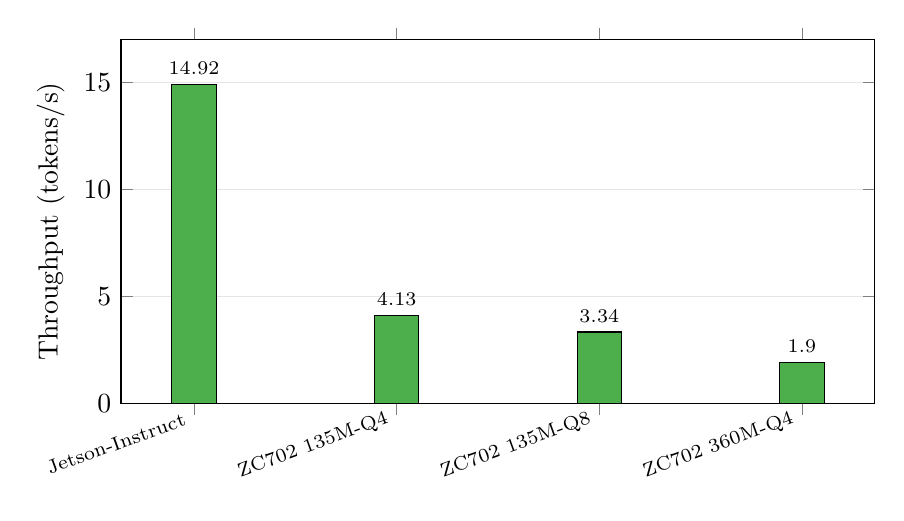
\begin{tikzpicture}
\begin{axis}[
  width=0.92\textwidth, height=6.2cm,
  ybar, bar width=16pt,
  ymin=0, ymax=17,
  ylabel={Throughput (tokens/s)},
  symbolic x coords={Jetson-Instruct,ZC702 135M-Q4,ZC702 135M-Q8,ZC702 360M-Q4},
  xtick=data, x tick label style={rotate=20,anchor=east,font=\scriptsize},
  nodes near coords, nodes near coords style={font=\scriptsize},
  enlarge x limits=0.12,
  ymajorgrids, grid style={gray!20}]
\addplot[fill=green!55!black!70] coordinates {
  (Jetson-Instruct,14.92)
  (ZC702 135M-Q4,4.13) (ZC702 135M-Q8,3.34) (ZC702 360M-Q4,1.90)};
\end{axis}
\end{tikzpicture}
\caption{Mean throughput across platforms and configurations. The Jetson GPU leads the ZC702 by
$\approx 3.6\times$ on the matched 135M-Q4 workload---consistent with its $\approx 10.7\times$ higher
clock and wider memory.}
\label{fig:p4-bars}
\end{figure}

\subsection{Evidence That the Deployment Is Memory-Bound}
\label{subsec:p4-membound}

The three ZC702 runs provide direct, two-axis evidence that throughput is limited by memory
movement, not arithmetic:

\begin{itemize}
  \item \textbf{Fixed network, wider weights (Q4 vs Q8).} The two configurations implement an
  \emph{identical} network and perform identical arithmetic per token; only the weight width differs.
  Q8 moves $\approx 1.5\times$ the bytes (156 vs 103\,MB) and runs $1.24\times$ slower (3.34 vs
  4.13 tok/s). A compute-bound design would show equal throughput.
  \item \textbf{Fixed weight width, larger network (135M vs 360M, both Q4).} The 360M model moves
  $\approx 2.4\times$ the bytes (248 vs 103\,MB) and runs at $0.46\times$ the throughput
  (1.90 vs 4.13 tok/s)---throughput falls in near-proportion to data volume.
\end{itemize}

Both observations are reconciled by the \emph{effective bandwidth} diagnostic
(throughput $\times$ bytes-per-token), which is approximately constant across three very different
models---the signature of a common memory ceiling (Table~\ref{tab:p4-membound},
Figure~\ref{fig:p4-membound}). The governing relationship is:
\[
\text{throughput (tok/s)} \;=\; \frac{\text{delivered DDR bandwidth (MB/s)}}{\text{bytes per token (MB)}}.
\]

\begin{table}[H]
\centering
\caption{Memory-bound evidence. Effective bandwidth (throughput $\times$ bytes/token) is nearly
constant; the separately-measured DDR read bandwidth is shown alongside.}
\label{tab:p4-membound}
\renewcommand{\arraystretch}{1.2}
\resizebox{\textwidth}{!}{%
\begin{tabular}{@{}lcccc@{}}
\toprule
\textbf{Configuration} & \textbf{Bytes/token} & \textbf{Throughput} & \textbf{Effective BW} & \textbf{Measured DDR read} \\
 & \textbf{(MB)} & \textbf{(tok/s)} & \textbf{(MB/s)} & \textbf{(MB/s)} \\
\midrule
SmolLM2-135M Q4 & 103 & 4.13 & 426 & 431 \\
SmolLM2-135M Q8 & 156 & 3.34 & 520 & 526 \\
SmolLM2-360M Q4 & 248 & 1.90 & 472 & 478 \\
\bottomrule
\end{tabular}}
\end{table}

\begin{figure}[H]
\centering
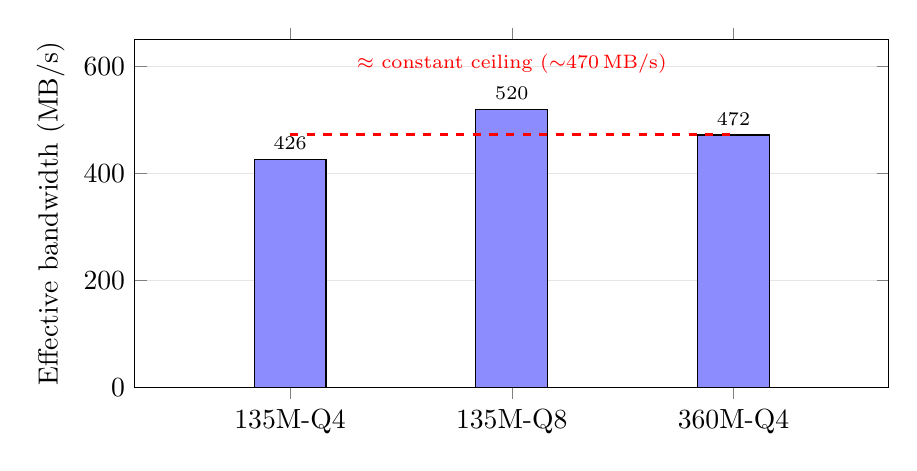
\begin{tikzpicture}
\begin{axis}[
  width=0.92\textwidth, height=6.0cm,
  ybar, bar width=26pt,
  ymin=0, ymax=650,
  ylabel={Effective bandwidth (MB/s)},
  symbolic x coords={135M-Q4,135M-Q8,360M-Q4},
  xtick=data,
  nodes near coords, nodes near coords style={font=\scriptsize},
  enlarge x limits=0.35,
  ymajorgrids, grid style={gray!20}]
\addplot[fill=blue!45] coordinates {(135M-Q4,426) (135M-Q8,520) (360M-Q4,472)};
\draw[red,thick,dashed] (axis cs:135M-Q4,473) -- (axis cs:360M-Q4,473);
\node[red,font=\scriptsize] at (axis cs:135M-Q8,605) {$\approx$ constant ceiling ($\sim$470\,MB/s)};
\end{axis}
\end{tikzpicture}
\caption{Effective bandwidth (throughput $\times$ bytes-per-token) stays near a common ceiling across
three different models, despite $2.4\times$ variation in bytes-per-token---the defining signature of a
memory-bound system. The mild rise for Q8 reflects its lower read-stall fraction (wider, more regular
INT8 reads versus INT4 nibble unpacking).}
\label{fig:p4-membound}
\end{figure}

\subsection{Output-Quality Assessment}
\label{subsec:p4-quality}

Throughput tells only half the story: a faster model is of little value if its answers are worse. To
place the three configurations on a quality axis, the 30 responses generated by each were graded
against ground truth on a simple three-point scale --- \textbf{2} for a correct and complete answer,
\textbf{1} for partially correct (the right method or some correct content but a flawed result), and
\textbf{0} for incorrect --- for a maximum of 60 points per model. The same rubric was applied to all
three, and the prompts with a definite answer (mathematics, factual science, geography) were graded
strictly. Table~\ref{tab:p4-quality} reports the totals.

\begin{table}[H]
\centering
\caption{Output-quality scores over the 30-prompt set (three-point scale; maximum 60).}
\label{tab:p4-quality}
\renewcommand{\arraystretch}{1.2}
\begin{tabular}{@{}lcl@{}}
\toprule
\textbf{Configuration} & \textbf{Score (/60)} & \textbf{Observation} \\
\midrule
SmolLM2-135M Q4 & 24 & Weakest; frequent incoherence and repetition. \\
SmolLM2-135M Q8 & 28 & $\approx$ Q4 (same network); small gain attributable to sampling. \\
SmolLM2-360M Q4 & 40 & Strongest; reasons soundly on several technical items. \\
\bottomrule
\end{tabular}
\end{table}

Two points follow. First, the 135M~Q4 and 135M~Q8 scores are close (24 versus 28): because they are
the \emph{same network} at different weight precision, their answer quality is essentially the same,
and the small difference lies within the noise of sampling --- which is exactly why the Q4/Q8 pair is
used for the bandwidth experiment of Section~\ref{subsec:p4-membound} and \emph{not} for quality
claims. Second, the 360M model scores markedly higher (40 versus 24), confirming that the quality
gain comes from \emph{parameter count}, at the cost of the $2.2\times$ slower generation reported
earlier.

\paragraph{A worked example.} The contrast is clearest on a factual prompt with a definite answer.
For GEO-03 --- \emph{``Which river is the longest in Africa and through which countries does it
flow?''}, whose answer is the Nile, running northward principally through Sudan and Egypt (with
headwaters reaching Uganda, South Sudan and Ethiopia) --- only the 360M model answered correctly
(Table~\ref{tab:p4-example}).

\begin{table}[H]
\centering
\caption{Verbatim responses to GEO-03 (the Nile), where only the largest model is correct.}
\label{tab:p4-example}
\renewcommand{\arraystretch}{1.3}
\begin{tabular}{@{}>{\raggedright\arraybackslash}p{0.15\textwidth} >{\raggedright\arraybackslash}p{0.63\textwidth} >{\centering\arraybackslash}p{0.08\textwidth}@{}}
\toprule
\textbf{Model} & \textbf{Response (verbatim, abridged)} & \textbf{Grade} \\
\midrule
135M Q4 &
``\dots\ flows through four countries: Egypt, Sudan, the Democratic Republic of the Congo, and the
Sudan. It originates in the Nile River, which is a tributary of the Indian Ocean.'' --- invents a
country the Nile does not cross, repeats Sudan, and makes the false claim that the Nile is a
tributary of the Indian Ocean.
& 0 \\
\midrule
135M Q8 &
``\dots\ flows through southern Egypt, Sudan, and parts of Kenya, Uganda, and South Sudan \dots\ the
fourth-longest river in the world, following the Nile in terms of length.'' --- the basin countries
are roughly right, but the answer contradicts itself (the Nile cannot be ``the fourth-longest \dots\
following the Nile'').
& 1 \\
\midrule
360M Q4 &
``The longest river in Africa is the Nile, which flows through Egypt and Sudan.'' --- correct and
concise, with no false statements.
& 2 \\
\bottomrule
\end{tabular}
\end{table}

Here the gradient is unambiguous. The 135M~Q4 answer is factually \emph{wrong}: it adds a country the
river does not cross and asserts that the Nile drains to the Indian Ocean. The 135M~Q8 answer is
\emph{closer} --- most of the named countries do lie in the Nile basin --- but it undercuts itself
with the self-contradictory claim that the Nile is ``the fourth-longest river \dots\ following the
Nile.'' Only the 360M~Q4 answer is \emph{correct}: brief, but free of error. This pattern --- the
smaller model confidently wrong, the larger model right --- recurs across the factual prompts and
accounts for most of the sixteen-point gap between the 135M and 360M scores. The larger model is thus
more reliable, though still not infallible, and outputs at this scale should be verified rather than
trusted.

\paragraph{A second example.} The same gap appears on a calculus prompt. For MATH-05 ---
\emph{``What is the integral of $1/(1+x^2)\,dx$?''}, whose answer is $\arctan(x)+C$ --- both 135M
models pursued entirely invalid methods, while only the 360M model identified the correct form
(Table~\ref{tab:p4-example2}).

\begin{table}[H]
\centering
\caption{Verbatim responses to MATH-05 (answer $\arctan(x)+C$): both small models use invalid
methods; only the largest identifies the arctangent form.}
\label{tab:p4-example2}
\renewcommand{\arraystretch}{1.3}
\begin{tabular}{@{}>{\raggedright\arraybackslash}p{0.15\textwidth} >{\raggedright\arraybackslash}p{0.63\textwidth} >{\centering\arraybackslash}p{0.08\textwidth}@{}}
\toprule
\textbf{Model} & \textbf{Response (verbatim, abridged)} & \textbf{Grade} \\
\midrule
135M Q4 &
``\dots\ rewrite the integral as the integral of 1/(1+x\textasciicircum 3) dx \dots\ 1/(1+x\textasciicircum 4) dx
\dots\ 1/(1+x\textasciicircum 12) dx.'' --- loops through ever-higher powers and never integrates.
& 0 \\
\midrule
135M Q8 &
``\dots\ take the logarithm of both sides \dots\ which transforms the integral into a logarithmic
integral \dots\ ln(1+x\textasciicircum 2) = x - x\textasciicircum(1/2).'' --- invents an invalid
logarithmic method.
& 0 \\
\midrule
360M Q4 &
``The integral of 1/(1+x\textasciicircum 2) is a classic example \dots\ specifically an integral of a
fundamental form known as the arctangent function.'' --- correctly identifies the result as the
arctangent (though the explicit formula it then writes is garbled).
& 1 \\
\bottomrule
\end{tabular}
\end{table}

Even here, where no model writes a clean $\arctan(x)+C$, the distinction is decisive: the two 135M
configurations are not merely imprecise but follow methods that cannot work --- an endless rewriting
of the exponent, and a non-existent ``logarithmic'' identity --- whereas the 360M model retrieves the
correct concept. Recognising \emph{what kind} of answer is required is itself a capability that
emerges with scale, and it is the main reason the larger model accumulates more partial- and
full-credit responses across the 30 prompts.

\subsection{The Efficiency Argument and Power Considerations}

The primary advantage of ztachip for edge deployment is not absolute throughput but energy
efficiency---tokens generated per watt. The Zynq-7020 at 93.75\,MHz with a 64-bit DDR bus is expected
to draw substantially less power than the Jetson GPU subsystem under load. A rigorous tokens-per-watt
comparison requires measured power on both platforms: on the ZC702, PMBus monitoring can report rail
currents (PL \texttt{VCCINT}, PS rails, DDR supply); on the Jetson, INA3221 sensors exposed through
sysfs provide per-rail current. These measurements are planned future work. The theoretical case for
ztachip efficiency rests on three points: (i) the FPGA fabric implements only the required logic,
avoiding unused general-purpose hardware; (ii) ztachip Pcores are purpose-built for the
matrix-multiply and activation operations that dominate LLM inference; and (iii) the deployment is
memory-bound, so power is dominated by the memory interface rather than excessive compute switching.

\subsubsection*{Vivado power estimate}

Pending rail-level measurement, a first-order power figure is available from Vivado's power analysis
of the implemented design. It is important to state its status precisely: this is a \emph{tool
estimate} produced by \emph{vectorless} analysis --- the switching activity is inferred from the
constraints rather than captured from a real workload --- and Vivado reports its confidence as
\emph{low}. It is therefore indicative, not a substitute for the measured power identified above as
future work. With that caveat, the estimated total on-chip power is \textbf{3.517\,W}, broken down in
Table~\ref{tab:p4-power}.

\begin{table}[H]
\centering
\caption{Vivado vectorless power estimate for the implemented design (XC7Z020 at 93.75\,MHz;
confidence: low). Shares are of the total on-chip power.}
\label{tab:p4-power}
\renewcommand{\arraystretch}{1.2}
\begin{tabular}{@{}lrr@{}}
\toprule
\textbf{Component} & \textbf{Power (W)} & \textbf{Share} \\
\midrule
PS7 (ARM cores + DDR controller) & 1.582 & 45.0\,\% \\
Block RAM (BRAM)                 & 0.610 & 17.3\,\% \\
Signals                          & 0.420 & 11.9\,\% \\
Clocks                           & 0.282 & 8.0\,\% \\
Logic                            & 0.237 & 6.7\,\% \\
MMCM (clock manager)             & 0.103 & 2.9\,\% \\
DSP                              & 0.044 & 1.3\,\% \\
I/O                              & $<$0.001 & $<$0.1\,\% \\
\midrule
Dynamic subtotal                 & 3.278 & 93.2\,\% \\
Device static                    & 0.239 & 6.8\,\% \\
\midrule
\textbf{Total on-chip}           & \textbf{3.517} & \textbf{100\,\%} \\
\bottomrule
\end{tabular}
\end{table}

Three features of the estimate are worth drawing out. First, the breakdown is \emph{dominated by the
memory and processor-system subsystem}: PS7 --- which contains the ARM cores and, crucially, the DDR
memory controller --- accounts for 1.582\,W (45\%), and Block RAM for a further 0.610\,W (17\%).
Together the memory-related blocks consume roughly three-fifths of the total, whereas the pure
compute logic (Logic plus DSP) draws only about 0.28\,W (8\%). This corroborates the memory-bound
finding of Section~\ref{subsec:p4-membound}: the design spends both its \emph{time} and its \emph{energy} chiefly on
moving data, not on arithmetic. Second, the dynamic component (3.278\,W, 93\%) far exceeds the static
leakage (0.239\,W, 7\%), as expected for a heavily utilised fabric. Third, the single MMCM appears
explicitly at 0.103\,W (3\%), consistent with the single-root clocking of
Section~\ref{subsec:p3-clock}. The analysis also reported a junction temperature of $65.6\,^{\circ}$C
at a $25\,^{\circ}$C ambient --- a comfortable thermal margin of roughly $19\,^{\circ}$C --- so the
design is in no danger of overheating.

As an order-of-magnitude indicator only, dividing the 4.13\,tok/s of the 135M\,Q4 configuration by
this 3.517\,W estimate gives $\approx 1.2$ tokens per second per watt. This figure should be read as
provisional: it rests on a low-confidence estimate and, until the Jetson is measured on the same
basis, does not by itself establish an efficiency advantage either way. Its value here is to give a
first quantitative anchor and to localise where the energy is spent.


